% latexmk -pdf theory.tex
\documentclass[11pt]{article}

\usepackage[margin=1in]{geometry}
\usepackage{amsmath,amssymb}
\usepackage{booktabs}
\usepackage{pgfplots}
\pgfplotsset{
  compat=1.18,
  blaxis/.style={
    width=0.84\textwidth,
    height=6.6cm,
    scale only axis,
    xmin=0.2, xmax=0.8,
    domain=0.2:0.8,
    samples=201,
    tick label style={font=\small},
    label style={font=\small},
    legend cell align=left,
    legend style={font=\small},
  },
}
\tikzset{
  declare function={
    sn(\t)=(\t-0.2)/0.6;
    krw(\t)=(sn(\t))^2;
    kro(\t)=(1-sn(\t))^2;
    lw(\t)=krw(\t);
    lo(\t)=0.5*kro(\t);
    ff(\t)=lw(\t)/(lw(\t)+lo(\t));
    df(\t)=((2*sn(\t)/0.6)*lo(\t)+lw(\t)*((1-sn(\t))/0.6))/((lw(\t)+lo(\t))^2);
  },
}
\usepackage[hidelinks]{hyperref}

\title{Fractional flow, the Welge shock,\\ and the saturation Jacobian}
\author{1D Buckley--Leverett notes}
\date{}

\begin{document}
\maketitle

\begin{abstract}
These notes derive the water fractional-flow function used by the solver, the Welge shock that makes the Buckley--Leverett solution single-valued, and the lower-bidiagonal Jacobian of the implicit upwind scheme.
The companion note \texttt{solver.tex} describes how that Jacobian, and the pressure system, are handed to AMGCL.
Capillary pressure and gravity are omitted: that is the classical Buckley--Leverett setting.
\end{abstract}

\section{Two-phase Darcy velocity}

Water and oil are immiscible and incompressible.
In one horizontal dimension, with no capillary pressure, both phases see the same pressure $p$.
Darcy's law is
\begin{equation}
\label{eq:darcy}
u_w = -k\lambda_w\frac{\partial p}{\partial x},
\qquad
u_o = -k\lambda_o\frac{\partial p}{\partial x},
\end{equation}
where $k$ is the absolute permeability and the phase mobilities are the relative permeability divided by the viscosity,
\begin{equation}
\label{eq:mobility}
\lambda_w = \frac{k_{rw}}{\mu_w},
\qquad
\lambda_o = \frac{k_{ro}}{\mu_o}.
\end{equation}
The total velocity and the total mobility are
\begin{equation}
\label{eq:total}
u_t = u_w + u_o = -k\lambda_t\frac{\partial p}{\partial x},
\qquad
\lambda_t = \lambda_w + \lambda_o.
\end{equation}
The fraction of the total stream that is water does not depend on $k$ or on the pressure gradient:
\begin{equation}
\label{eq:f-def}
f = \frac{u_w}{u_t} = \frac{\lambda_w}{\lambda_w + \lambda_o}.
\end{equation}
Thus $u_w = f\, u_t$.
The function $f$ is the fractional-flow function.
It depends on water saturation $S$ only through the relative permeabilities.

Adding the two phase mass balances, and using incompressibility, gives
\begin{equation}
\label{eq:div-ut}
\frac{\partial u_t}{\partial x} = 0
\end{equation}
wherever there are no wells.
In one dimension the total velocity is therefore uniform in $x$.
A prescribed inlet rate fixes it in time as well.
Permeability may still vary with $x$: it changes the pressure drop required to push that rate, through~\eqref{eq:total}, but it does not appear in the saturation equation derived next.

\section{The Buckley--Leverett equation}

Water conservation with constant porosity $\phi$, the starting point of Buckley and Leverett~\cite{buckley1942}, is
\begin{equation}
\label{eq:water-balance}
\phi\frac{\partial S}{\partial t} + \frac{\partial u_w}{\partial x} = 0.
\end{equation}
Substitute $u_w = f(S)\, u_t$.
On a core of length $L$ with constant $u_t > 0$, the dimensionless coordinates
\begin{equation}
\label{eq:dimensionless}
x_D = \frac{x}{L},
\qquad
t_D = \frac{1}{\phi L}\int_0^t u_t(\tau)\,d\tau
\end{equation}
remove $\phi$, $L$, and the rate.
The integral $t_D$ is the number of pore volumes injected.
Dropping the subscript $D$,~\eqref{eq:water-balance} becomes
\begin{equation}
\label{eq:bl}
\frac{\partial S}{\partial t} + \frac{\partial f(S)}{\partial x} = 0,
\qquad x\in(0,1).
\end{equation}
The program integrates~\eqref{eq:bl}.
The initial core is at connate water, and the inlet stream is water at the maximum water saturation:
\begin{equation}
\label{eq:icbc}
S(x,0) = S_{wc},
\qquad
S(0,t) = S_{\max} = 1 - S_{or}.
\end{equation}
At $S_{\max}$ the oil relative permeability vanishes, so $f(S_{\max}) = 1$.
At $S_{wc}$ the water relative permeability vanishes, so $f(S_{wc}) = 0$.

\section{Corey mobilities and $f'(S)$}

Normalized saturation maps the mobile range onto $[0,1]$:
\begin{equation}
\label{eq:sn}
s = \frac{S - S_{wc}}{1 - S_{wc} - S_{or}},
\qquad
\frac{ds}{dS} = \frac{1}{1 - S_{wc} - S_{or}}.
\end{equation}
Corey relative permeabilities~\cite{corey1954} with endpoint values $k_{rw}^{0}$ and $k_{ro}^{0}$ are
\begin{equation}
\label{eq:corey}
k_{rw} = k_{rw}^{0}\, s^{n_w},
\qquad
k_{ro} = k_{ro}^{0}\, (1-s)^{n_o}.
\end{equation}
Write $A_w = k_{rw}^{0}/\mu_w$ and $A_o = k_{ro}^{0}/\mu_o$.
Inside $(0,1)$ in $s$,
\begin{align}
\lambda_w &= A_w s^{n_w},
&
\frac{d\lambda_w}{dS} &= A_w n_w s^{n_w-1}\frac{ds}{dS},
\label{eq:dlw}\\
\lambda_o &= A_o (1-s)^{n_o},
&
\frac{d\lambda_o}{dS} &= -A_o n_o (1-s)^{n_o-1}\frac{ds}{dS}.
\label{eq:dlo}
\end{align}
Differentiating the quotient~\eqref{eq:f-def} gives the chain-rule identity used by both the Welge solver and the Newton matrix:
\begin{equation}
\label{eq:df}
f'(S)
=
\frac{
\lambda_w'(S)\,\lambda_o(S) - \lambda_w(S)\,\lambda_o'(S)
}{
\bigl(\lambda_w(S)+\lambda_o(S)\bigr)^2
}.
\end{equation}
For $n_w>1$ and $n_o>1$ the derivatives vanish at the endpoints, so $f'(S_{wc}) = f'(S_{\max}) = 0$.
The default data in the program are
\begin{equation}
\label{eq:defaults}
S_{wc} = S_{or} = 0.2,
\quad
n_w = n_o = 2,
\quad
k_{rw}^{0} = k_{ro}^{0} = 1,
\quad
\mu_w = 1,
\quad
\mu_o = 2.
\end{equation}
The endpoint mobility ratio is then
\begin{equation}
\label{eq:M}
M = \frac{A_w}{A_o} = \frac{k_{rw}^{0}/\mu_w}{k_{ro}^{0}/\mu_o} = 2.
\end{equation}
With these exponents, $f$ leaves $S_{wc}$ with zero slope, steepens, and flattens again at $S_{\max}$.
That S-shape is what forces a shock.
Figure~\ref{fig:kr} is the relative-permeability plot for this Corey model, in the role of Buckley and Leverett's Figure~1.
Figure~\ref{fig:ff} is the matching fractional-flow plot, in the role of their Figure~2, including the viscosity ratio $\mu_o/\mu_w = 2$.
The curves are the default data~\eqref{eq:defaults}, not a tracing of the measured unconsolidated sand in that paper.
On Figure~\ref{fig:ff}, $f'$ is drawn on its own scale.
It is zero at both endpoints, peaks between them, and is already decreasing at the Welge saturation $S_f$ marked on the plot.
The dotted segment is the chord from $(S_{wc},0)$ that is tangent to $f$ at $S_f$.

\begin{figure}[ht]
\centering
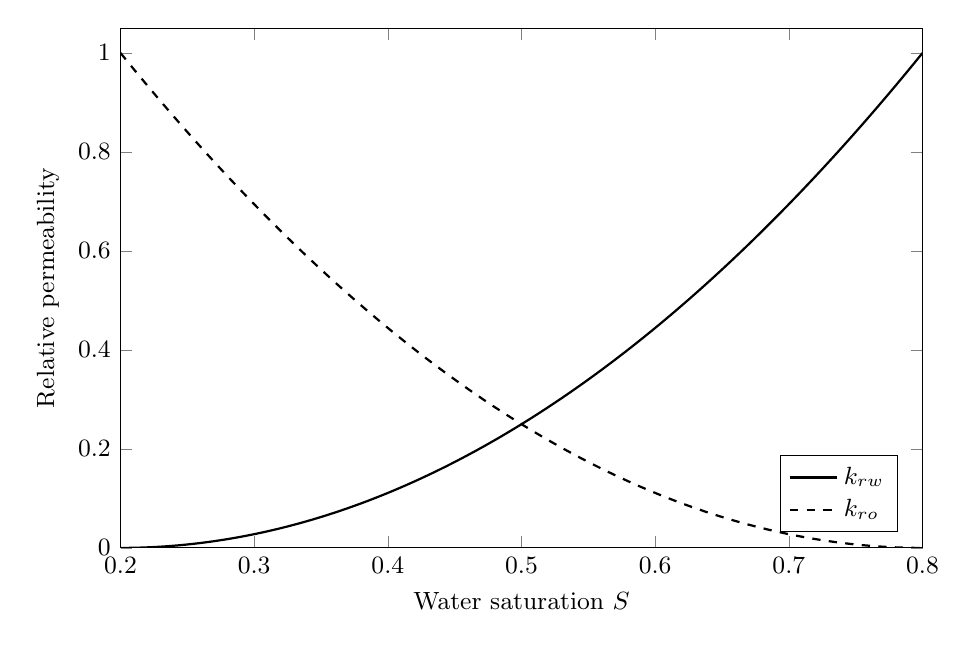
\begin{tikzpicture}
\begin{axis}[
  blaxis,
  xlabel={Water saturation $S$},
  ylabel={Relative permeability},
  ymin=0, ymax=1.05,
  legend pos=south east,
]
\addplot[thick] {krw(x)};
\addlegendentry{$k_{rw}$}
\addplot[thick, dashed] {kro(x)};
\addlegendentry{$k_{ro}$}
\end{axis}
\end{tikzpicture}
\caption{Corey relative permeabilities for $n_w = n_o = 2$, $S_{wc} = S_{or} = 0.2$, and unit endpoints.
This is the same arrangement as Figure~1 of Buckley and Leverett~\cite{buckley1942}.}
\label{fig:kr}
\end{figure}

\begin{figure}[ht]
\centering
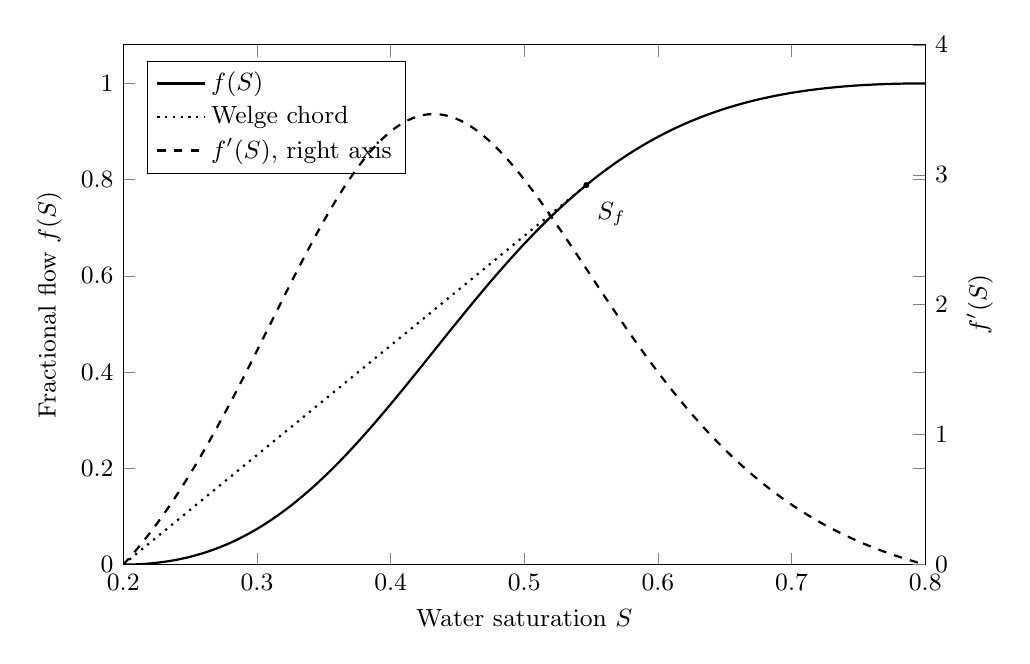
\begin{tikzpicture}
\begin{axis}[
  blaxis,
  xlabel={Water saturation $S$},
  ylabel={Fractional flow $f(S)$},
  ymin=0, ymax=1.08,
  legend pos=north west,
]
\addplot[thick] {ff(x)};
\addlegendentry{$f(S)$}
\addplot[dotted, thick, domain=0.2:0.54641] {2.27671*(x-0.2)};
\addlegendentry{Welge chord}
\addlegendimage{thick, dashed}
\addlegendentry{$f'(S)$, right axis}
\fill (axis cs:0.54641,0.7887) circle (1.1pt);
\node[anchor=north west, font=\small, inner sep=1pt] at (axis cs:0.552,0.76) {$S_f$};
\end{axis}
\begin{axis}[
  blaxis,
  ymin=0, ymax=4,
  ylabel={$f'(S)$},
  axis y line*=right,
  axis x line=none,
  xtick=\empty,
]
\addplot[thick, dashed] {df(x)};
\end{axis}
\end{tikzpicture}
\caption{Fractional flow and $f'(S)$ for the default Corey data and $\mu_o/\mu_w = 2$.
This is the same arrangement as Figure~2 of Buckley and Leverett~\cite{buckley1942}.
The chord meets $f$ at $S_f = 0.54641$, where $f'(S_f)$ equals the chord slope.}
\label{fig:ff}
\end{figure}

One consequence of the same mobilities is used only by the pressure solution.
For $n_w = n_o = 2$,
\[
\lambda_t(s) = A_w s^2 + A_o(1-s)^2
\]
has a minimum at $s = A_o/(A_w+A_o) = 1/3$, where $\lambda_t = 1/3$.
That value is below both endpoint mobilities $\lambda_t(0) = A_o = 1/2$ and $\lambda_t(1) = A_w = 1$.
A fixed total rate therefore needs a larger pressure drop once both phases are mobile.
The inlet pressure in the run rises for that reason.

\section{Characteristics and the multi-valued profile}

Equation~\eqref{eq:bl} is a scalar conservation law.
If $f'$ is evaluated on a smooth solution, saturation is constant along characteristics
\begin{equation}
\label{eq:char}
\frac{dx}{dt} = f'(S).
\end{equation}
From the inlet state $S_{\max}$, whose characteristic speed is $f'(S_{\max}) = 0$, a centered rarefaction would assign to each speed $\xi = x/t$ the saturation satisfying $f'(S) = \xi$.
Because $f'$ increases from $0$ at $S_{wc}$ and then decreases back to $0$ at $S_{\max}$, the same speed $\xi$ is attained at two saturations.
The formal rarefaction is multi-valued.
The physical solution replaces the folded part by a discontinuity.

\section{The Welge tangent}

A discontinuity from left state $S_l$ to right state $S_r$, with $f_r = f(S_r)$, travels at the Rankine--Hugoniot speed
\begin{equation}
\label{eq:rh}
v = \frac{f(S_l) - f(S_r)}{S_l - S_r}.
\end{equation}
Ahead of the waterflood the right state is the initial saturation, $S_r = S_{wc}$ and $f(S_{wc}) = 0$, so
\begin{equation}
\label{eq:chord}
v(S) = \sigma(S) = \frac{f(S)}{S - S_{wc}}.
\end{equation}
This is the slope of the chord from $(S_{wc}, 0)$ to $(S, f(S))$.
Not every chord is admissible.
Characteristics must run into the shock, and the chord must lie above the graph of $f$ between $S_{wc}$ and the shock saturation $S_f$ (the Oleinik condition~\cite{oleinik1959} for a convex flux, applied here to the convex hull of an S-shaped flux).
For the standard fractional-flow curve those requirements select the chord of \emph{largest} slope.
Differentiating~\eqref{eq:chord},
\begin{equation}
\label{eq:sigma-prime}
\sigma'(S)
=
\frac{f'(S)\,(S-S_{wc}) - f(S)}{(S-S_{wc})^2},
\end{equation}
so a stationary point of $\sigma$ satisfies
\begin{equation}
\label{eq:welge}
g(S_f) = 0,
\qquad
g(S) = f'(S)\,(S - S_{wc}) - f(S).
\end{equation}
Equivalently,
\begin{equation}
\label{eq:tangent}
f'(S_f) = \frac{f(S_f)}{S_f - S_{wc}} = v_s.
\end{equation}
The chord is tangent to $f$ at $S_f$.
That is Welge's construction~\cite{welge1952}, drawn as the dotted segment in Figure~\ref{fig:ff}.
The shock speed $v_s$ is both the characteristic speed just behind the shock and the Rankine--Hugoniot speed of the jump from $S_f$ down to $S_{wc}$.
The program finds $S_f$ by a golden-section search for the maximum of $\sigma$, then polishes the root of $g$ by a scalar Newton iteration.
With the default data,
\[
S_f = 0.54641,
\qquad
v_s = 2.27671,
\qquad
t_{\mathrm{bt}} = 1/v_s = 0.43923.
\]
The tangent residual $f'(S_f) - v_s$ comes out at roundoff.

The equal-area (Welge) statement is the same fact drawn on the graph of $f$: the tangent from $(S_{wc},0)$ cuts off the concave part of $f$, and the shock jumps from $S_{wc}$ to the point of tangency.
Behind that point the graph itself is already the convex hull, so the solution is a rarefaction rather than a second shock.

\section{The entropy solution sampled by the program}

After the shock, $f'$ decreases from $v_s$ at $S_f$ to $0$ at $S_{\max}$.
The self-similar solution at a fixed $t>0$ is therefore
\begin{equation}
\label{eq:exact}
S(x,t) =
\begin{cases}
S^{\sharp}(x/t), & 0 \le x/t < v_s,\\
S_{wc}, & x/t \ge v_s,
\end{cases}
\end{equation}
where $S^{\sharp}(\xi)$ is the unique saturation in $[S_f, S_{\max}]$ with
\begin{equation}
\label{eq:rarefaction}
f'\bigl(S^{\sharp}(\xi)\bigr) = \xi.
\end{equation}
The program inverts~\eqref{eq:rarefaction} by bisection: if $f'(S_{\mathrm{mid}}) > \xi$, the trial saturation is still too small, because $f'$ is decreasing on that interval.
The shock position is the characteristic $x_s(t) = v_s t$.
It reaches the outlet at the breakthrough time $t_{\mathrm{bt}} = 1/v_s$.
The default run stops at $t = 0.55/v_s$, so the exact shock is at $x = 0.55$, inside the domain and on the downstream edge of the tight streak.

\section{Implicit upwind residual}

Cells are centered at $x_i = (i+\tfrac12)\Delta x$, $i = 0,\ldots,N-1$, with $\Delta x = 1/N$.
Integrate~\eqref{eq:bl} over cell $i$ and one time step.
The accumulation is $\Delta x\,(S_i - S_i^n)$.
The interface fluxes are $f$ evaluated upstream.
Flow is in the positive $x$ direction, so the upstream neighbor of face $i+\tfrac12$ is cell $i$:
\begin{equation}
\label{eq:flux}
F_{i+1/2} = f(S_i),
\qquad
F_{-1/2} = f(S_{\max}) = 1.
\end{equation}
Backward Euler then gives the residual whose root is the new saturation.
For the inlet cell and for every later cell,
\begin{equation}
\label{eq:residual}
\begin{aligned}
R_0 &= \frac{\Delta x}{\Delta t}\bigl(S_0 - S_0^n\bigr) + f(S_0) - 1,\\
R_i &= \frac{\Delta x}{\Delta t}\bigl(S_i - S_i^n\bigr) + f(S_i) - f(S_{i-1}),
\quad i = 1,\ldots,N-1.
\end{aligned}
\end{equation}
The scheme is conservative.
Summing~\eqref{eq:residual} over the grid, interior fluxes cancel and
\begin{equation}
\label{eq:conservation}
\sum_{i=0}^{N-1}(S_i - S_{wc})\,\Delta x
=
t - \sum_{\mathrm{steps}} f(S_{N-1}^{n+1})\,\Delta t,
\end{equation}
which is injected volume minus produced volume.
The second sum uses the new saturation because the time integrator is backward Euler.
The program checks~\eqref{eq:conservation} to about $10^{-15}$.

\section{The bidiagonal Jacobian}

Newton's method solves $R(S) = 0$.
One iteration computes a correction $\delta$ from
\begin{equation}
\label{eq:newton}
J(S)\,\delta = -R(S),
\qquad
J_{ij} = \frac{\partial R_i}{\partial S_j},
\end{equation}
then sets $S \leftarrow S + \delta$, with a line search and a clamp onto $[S_{wc}, S_{\max}]$ as described in the solver note.

Only two entries in row $i$ are nonzero.
From~\eqref{eq:residual} and the chain rule~\eqref{eq:df},
\begin{equation}
\label{eq:jacobian}
J_{i,i} = \frac{\Delta x}{\Delta t} + f'(S_i),
\qquad
J_{i,i-1} = -f'(S_{i-1})\ \ (i \ge 1).
\end{equation}
Every other derivative is zero.
The inlet residual does not depend on an unknown upstream saturation, so row $0$ contains only the diagonal.
The matrix is lower bidiagonal:
\begin{equation}
\label{eq:bidiagonal}
J =
\begin{pmatrix}
a_0 & & & \\
-b_1 & a_1 & & \\
& -b_2 & a_2 & \\
& & \ddots & \ddots
\end{pmatrix},
\quad
\begin{aligned}
a_i &= \Delta x/\Delta t + f'(S_i),\\
b_i &= f'(S_{i-1}).
\end{aligned}
\end{equation}
On the physical range of this flood, $f' \ge 0$, so the diagonal is positive and the subdiagonal is nonpositive.
$J$ is a nonsymmetric M-matrix.
It is not symmetric, so conjugate gradients are the wrong iteration; the program uses BiCGStab.
It is bidiagonal, so an ILU(0) factorization that keeps only the original nonzeros is already the exact LU.
That is why the transport solve reports one iteration once AMGCL's ILU(0) relaxation is used inside the preconditioner.
The pressure matrix derived in the companion note is tridiagonal and symmetric, and that is the system on which the multigrid cycle does real work.

If a capillary term $-\partial_x\bigl(\varepsilon(S)\partial_x S\bigr)$ were added, each residual would also depend on $S_{i+1}$ and $J$ would be tridiagonal.
The classical Buckley--Leverett problem has no such term, and the code does not add one.

\begin{thebibliography}{9}

\bibitem{buckley1942}
S.~E. Buckley and M.~C. Leverett.
\newblock Mechanism of fluid displacement in sands.
\newblock \emph{Transactions of the AIME}, 146:107--116, 1942.

\bibitem{corey1954}
A.~T. Corey.
\newblock The interrelation between gas and oil relative permeabilities.
\newblock \emph{Producers Monthly}, 19(1):38--41, 1954.

\bibitem{oleinik1959}
O.~A. Oleinik.
\newblock Uniqueness and stability of the generalized solution of the Cauchy problem for a quasi-linear equation.
\newblock \emph{Uspekhi Matematicheskikh Nauk}, 14(2):165--170, 1959.

\bibitem{welge1952}
H.~J. Welge.
\newblock A simplified method for computing oil recovery by gas or water drive.
\newblock \emph{Transactions of the AIME}, 195:91--98, 1952.

\end{thebibliography}

\end{document}
